%\VignetteIndexEntry{UsingDDGExplorer} 

% This file was converted to LaTeX by Writer2LaTeX ver. 1.2
% see http://writer2latex.sourceforge.net for more info

% Conversion and modifications by Luis Perez 17-Jul-2014
\documentclass[letterpaper]{article}
\usepackage[utf8]{inputenc}
\usepackage[T1]{fontenc}
\usepackage[english]{babel}
\usepackage{amsmath}
\usepackage{amssymb,amsfonts,textcomp}
\usepackage{color}
\usepackage{array}
\usepackage{supertabular}
\usepackage{hhline}
\usepackage{hyperref}
\hypersetup{pdftex, colorlinks=true, linkcolor=blue, citecolor=blue, filecolor=blue, urlcolor=blue, pdftitle=}
\usepackage[pdftex]{graphicx}
% Outline numbering
\setcounter{secnumdepth}{0}
\makeatletter
\newcommand\arraybslash{\let\\\@arraycr}
\makeatother
% List styles
\newcommand\liststyleWWviiiNumii{%
\renewcommand\labelitemi{•}
\renewcommand\labelitemii{•}
\renewcommand\labelitemiii{•}
\renewcommand\labelitemiv{•}
}
\newcommand\liststyleWWviiiNumiii{%
\renewcommand\labelitemi{•}
\renewcommand\labelitemii{•}
\renewcommand\labelitemiii{•}
\renewcommand\labelitemiv{•}
}
\newcommand\liststyleWWviiiNumiv{%
\renewcommand\labelitemi{←}
\renewcommand\labelitemii{•}
\renewcommand\labelitemiii{•}
\renewcommand\labelitemiv{•}
}
\newcommand\liststyleWWviiiNumv{%
\renewcommand\labelitemi{•}
\renewcommand\labelitemii{•}
\renewcommand\labelitemiii{•}
\renewcommand\labelitemiv{•}
}
\newcommand\liststyleWWviiiNumvi{%
\renewcommand\labelitemi{←}
\renewcommand\labelitemii{•}
\renewcommand\labelitemiii{•}
\renewcommand\labelitemiv{•}
}
\newcommand\liststyleWWviiiNumvii{%
\renewcommand\labelitemi{•}
\renewcommand\labelitemii{•}
\renewcommand\labelitemiii{•}
\renewcommand\labelitemiv{•}
}
\newcommand\liststyleWWviiiNumix{%
\renewcommand\theenumi{\arabic{enumi}}
\renewcommand\theenumii{\arabic{enumii}}
\renewcommand\theenumiii{\arabic{enumiii}}
\renewcommand\theenumiv{\arabic{enumiv}}
\renewcommand\labelenumi{\theenumi.}
\renewcommand\labelenumii{\theenumii.}
\renewcommand\labelenumiii{\theenumiii.}
\renewcommand\labelenumiv{\theenumiv.}
}
% Page layout (geometry)
\setlength\voffset{-1in}
\setlength\hoffset{-1in}
\setlength\topmargin{0.5in}
\setlength\oddsidemargin{1in}
\setlength\textheight{8.1779995in}
\setlength\textwidth{6.5in}
\setlength\footskip{0.76100004in}
\setlength\headheight{0.5in}
\setlength\headsep{0.461in}
% Footnote rule
\setlength{\skip\footins}{0.0469in}
\renewcommand\footnoterule{\vspace*{-0.0071in}\setlength\leftskip{0pt}\setlength\rightskip{0pt plus 1fil}\noindent\textcolor{black}{\rule{0.25\columnwidth}{0.0071in}}\vspace*{0.0398in}}
% Pages styles
\makeatletter
\newcommand\ps@Standard{
  \renewcommand\@oddhead{Using the DDG Explorer}
  \renewcommand\@evenhead{Using the DDG Explorer}
  \renewcommand\@oddfoot{\thepage{}}
  \renewcommand\@evenfoot{\thepage{}}
  \renewcommand\thepage{\arabic{page}}
}
\newcommand\ps@FirstPage{
  \renewcommand\@oddhead{}
  \renewcommand\@evenhead{\@oddhead}
  \renewcommand\@oddfoot{}
  \renewcommand\@evenfoot{\@oddfoot}
  \renewcommand\thepage{\arabic{page}}
}
\makeatother
\pagestyle{Standard}
\setlength\tabcolsep{1mm}
\renewcommand\arraystretch{1.3}
\title{}
\begin{document}
\clearpage\setcounter{page}{1}\pagestyle{Standard}
\thispagestyle{FirstPage}
\section{Using the DDG Explorer}
\subsection{Barbara Lerner, Emery Boose}
\subsection{December 2013}
\subsection{What is the DDG Explorer?}
{\mdseries\upshape\color{black}
The DDG Explorer is a tool that allows the user to view and query the Data Derivation Graphs (DDGs) that are created by running programs that collect this data derivation information as they execute. \ The focus of this document is on its use with DDGs created from execution of instrumented R scripts. \ Currently, DDGs can also be created through execution of Little-JIL processes. \ The DDG notation is general enough to support many languages, but there are currently no other implementations.}

{\mdseries\upshape\color{black}
DDG Explorer has the following functionality:}

\liststyleWWviiiNumii
\begin{itemize}
\item {\color{black}
Visualization of DDGs, with the ability to zoom in and out to selectively show or hide details.}
\item {\color{black}
Ability to view the data or R functions referenced by pieces of the DDG}
\item {\color{black}
Ability to query a DDG to discover how an input data value gets used, or what data and processing steps lead to the derivation of a particular output value}
\item {\color{black}
Ability to compare R scripts used to generate different DDGs}
\item {\color{black}
Ability to search for where a particular data file is used or generated.}
\end{itemize}
{\mdseries\upshape\color{black}
An overview of the project that DDG Explorer was developed in is available at http://www.mtholyoke.edu/\~{}blerner/DataProvenance/.}

\subsection{Downloading DDG Explorer}
{\mdseries\upshape\color{black}
The DDG Explorer software can be downloaded from:}

{\mdseries\upshape\color{black}
http://www.mtholyoke.edu/\~{}blerner/DataProvenance/code/ddg-explorer.jar}

{\mdseries\upshape\color{black}
Required software: \ }

\liststyleWWviiiNumii
\begin{itemize}
\item {\color{black}
DDG Explorer requires Java 1.7. \ Most computers come with Java installed, but if you do not have it, you can download it from \url{http://www.oracle.com/technetwork/java/javase/downloads/index.html}. \ Be sure to select JRE and then the version appropriate for your operating system.}
\end{itemize}
\subsection{Starting the DDG Explorer}
{\mdseries\upshape\color{black}
After downloading DDGExplorer.jar, you should be able to start it by double-clicking on the icon.}

\subsection{Loading a DDG from a File}
{\mdseries\upshape\color{black}
When DDG Explorer starts, you should see a window that looks like this:}

 \includegraphics[width=6.5in,height=2.889in]{UsingDDGExplorer-img/UsingDDGExplorer-img001.png} 

{\mdseries\upshape\color{black}
Across the top of this window, you should see 4 buttons:}

\liststyleWWviiiNumii
\begin{itemize}
\item {\color{black}
Load from file}
\item {\color{black}
Load from database}
\item {\color{black}
Compare R scripts}
\item {\color{black}
Find Data Files}
\end{itemize}
{\mdseries\upshape\color{black}
The large empty area is used to display error messages or other informational messages as necessary.}

{\mdseries\upshape\color{black}
The DDG Explorer stores its data in a database (details in the Behind the scenes section below if you are interested). \ The Load from Database, Compare R Scripts, and Find Data Files buttons only do useful things once there are DDGs in the database. To get data into the database, you must first load it from a file and then save it to the database.}

{\mdseries\upshape\color{black}
When you click on Load from File, you will be presented with a standard file browser. \ Exactly how this file browser looks will depend on the operating system that you are using. \ Using the file browser, you should navigate to a ddg.txt file, select that and click Open. \ The ddg.txt is located in the DDG directory used by the R script. \ The location of the directory is defined by the ddg.path variable defined at the top of the R script.}

\subsection{The DDG window}
{\mdseries\upshape\color{black}
After opening a ddg.txt file, you will see a window that looks like this:}

 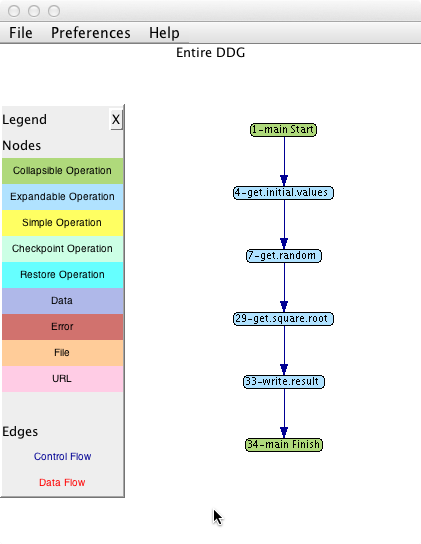
\includegraphics[width=3.472in,height=4.4866in]{UsingDDGExplorer-img/UsingDDGExplorer-img002.png} 

{\mdseries\upshape\color{black}
Along the top of the window are 3 menus: \ File, Preferences and Help. \ On the left side is a legend that explains the colors used in the DDG. \ On the right is the initial view of the DDG in a collapsed state.}

{\mdseries\upshape\color{black}
A DDG is drawn as a number of nodes (the oval shapes) connected with edges (the arrows). \ The nodes represent either data or processing steps, while the edges show how execution goes from one processing step to the next, or how data is used or produced by a processing step.}

{\mdseries\upshape\color{black}
For example, the DDG as drawn above corresponds to the following pieces of R code:}

{\color{black}
get.initial.values()}

{\mdseries\upshape\color{black}
estimate {\textless}- get.random(number)}


\bigskip

{\mdseries\upshape\color{black}
\# Begin get.square.root}

{\mdseries\upshape\color{black}
check {\textless}- number}

{\mdseries\upshape\color{black}
\textcolor[rgb]{0.49803922,0.0,0.37254903}{while} (check \textcolor[rgb]{0.62352943,0.24705882,0.49803922}{{\textgreater}} \textcolor[rgb]{0.0,0.0,0.49803922}{0}) \{}

{\mdseries\upshape\color{black}
\ \ \# repeat calculation until tests OK}

{\mdseries\upshape\color{black}
\ \ estimate {\textless}- calc.square.root(number,estimate)}

{\mdseries\upshape\color{black}
\ \ difference {\textless}- get.difference(number,estimate)}

{\mdseries\upshape\color{black}
\ \ check {\textless}- get.check.value(difference,tolerance)}

{\mdseries\upshape\color{black}
\}}

{\mdseries\upshape\color{black}
sqr.root {\textless}- store.result(number,estimate)}

{\mdseries\upshape\color{black}
\# End get.square.root}


\bigskip

{\mdseries\upshape\color{black}
write.result({\textquotedbl}sqr-root.csv{\textquotedbl},sqr.root)}

{\mdseries\upshape\color{black}
The exact nodes that are drawn are based on the instrumentation that was placed in the code. \ (See the Using the R DDG Library document to learn how to do this best.) \ Here is the same code with the instrumentation added.}

{\color{black}
ddg.start({\textquotedbl}main{\textquotedbl})}


\bigskip

{\mdseries\upshape\color{black}
ddg.start({\textquotedbl}get.initial.values{\textquotedbl})}

{\mdseries\upshape\color{black}
get.initial.values()}

{\mdseries\upshape\color{black}
ddg.finish({\textquotedbl}get.initial.values{\textquotedbl})}


\bigskip

{\mdseries\upshape\color{black}
ddg.start({\textquotedbl}get.random{\textquotedbl})}

{\mdseries\upshape\color{black}
estimate {\textless}- get.random(number)}

{\mdseries\upshape\color{black}
ddg.finish({\textquotedbl}get.random{\textquotedbl})}


\bigskip

{\mdseries\upshape\color{black}
ddg.start({\textquotedbl}get.square.root{\textquotedbl})}


\bigskip

{\mdseries\upshape\color{black}
check {\textless}- number}


\bigskip

{\mdseries\upshape\color{black}
while (check {\textgreater} 0) \{}

{\mdseries\upshape\color{black}
\ \ ddg.start({\textquotedbl}get.next.estimate{\textquotedbl})}


\bigskip

{\mdseries\upshape\color{black}
\ \ \# repeat calculation until tests OK}

{\mdseries\upshape\color{black}
\ \ estimate {\textless}- calc.square.root(number,estimate)}

{\mdseries\upshape\color{black}
\ \ difference {\textless}- get.difference(number,estimate)}

{\mdseries\upshape\color{black}
\ \ check {\textless}- get.check.value(difference,tolerance)}


\bigskip

{\mdseries\upshape\color{black}
\ \ ddg.finish({\textquotedbl}get.next.estimate{\textquotedbl})}

{\mdseries\upshape\color{black}
\}}


\bigskip

{\mdseries\upshape\color{black}
ddg.finish({\textquotedbl}get.square.root{\textquotedbl})}


\bigskip

{\mdseries\upshape\color{black}
ddg.start({\textquotedbl}write.result{\textquotedbl})}

{\mdseries\upshape\color{black}
sqr.root {\textless}- store.result(number,estimate)}

{\mdseries\upshape\color{black}
write.result({\textquotedbl}sqr-root.csv{\textquotedbl},sqr.root)}

{\mdseries\upshape\color{black}
ddg.finish({\textquotedbl}write.result{\textquotedbl})}


\bigskip

{\mdseries\upshape\color{black}
ddg.finish({\textquotedbl}main{\textquotedbl})}

{\mdseries\upshape\color{black}
Each ddg.start()...ddg.finish() pair identifies a number of nodes that can be collapsed into a single node. \ This allows the user to zoom in and out on the detail. \ In the initial drawing, the “main” node is expanded (resulting in a pair of green nodes labeled “main Start” and “main Finish”), while the remaining nodes are “collapsed” (drawn in blue). \ The user can single-click on a blue node to expand it. \ For example, if the user clicks on the get.square.root node, the DDG is redrawn as:}

 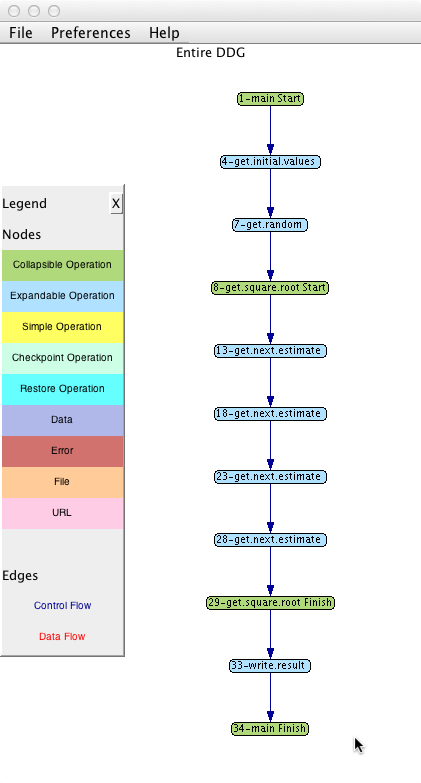
\includegraphics[width=3.8083in,height=7.0835in]{UsingDDGExplorer-img/UsingDDGExplorer-img003.png} 

{\mdseries\upshape\color{black}
Single-clicking on either the get.square.root Start node or the get.square.root Finish node would return to the original view of the DDG. \ To see the entire DDG, click on the top Start node to collapse the DDG to a single node. \ Then right-click and select “Expand All”.}

{\mdseries\upshape\color{black}
A Simple Operation (drawn as a yellow node) represents a processing step that the user cannot zoom in on. \ It represents the lowest level of processing captured by the DDG. \ Below is a view of the DDG where we have expanded the get.initial.values step. \ Here you can see a simple operation, named “3-get.initial.values”. \ We also see 2 lilac-colored nodes. \ These nodes represent data. \ In this case, the get.initial.values operation is setting a variable named “number” and another variable named “tolerance”. \ We can tell that get.initial.values is setting these values since the arrow points from the Operation node to the Data nodes. \ The number variable is used in the operations get.random, get.square.root and write.result. \ Similarly, tolerance is used by get.square.root. \ Here, we can tell that these operations are using the data because the arrows point from the data to the operations, signifying that the data are inputs to those operations.}

 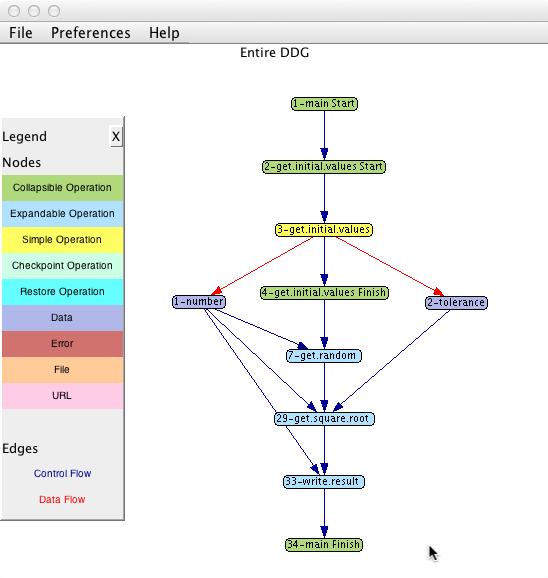
\includegraphics[width=5.9654in,height=6.2917in]{UsingDDGExplorer-img/UsingDDGExplorer-img004.png} 

{\mdseries\upshape\color{black}
There are two additional types of operation nodes: \ Checkpoint Operation and Restore Operation. \ A Checkpoint Operation node is created when the user calls the ddg.checkpoint function. \ It will have an output that is a node representing the RData file that holds the R workspace objects at that point in time. \ A Restore Operation node is created when the user calls ddg.restore. \ It will have an input which is the RData file being restored. \ These node types are not used in this example.}

{\mdseries\upshape\color{black}
There are three additional data node types: \ File, URL and Error. \ The lilac color indicates a data value stored in memory, either a simple value like a number or character, or a more complex value like a vector or data frame. \ A File node signifies that the data are stored in a file, while a URL node indicates that the data came from a website. \ An Error node (in red) represents an error during execution of the R script that caused the script to fail.}

{\color{black}
Scrolling, magnifying, clicking, right-clicking}

{\mdseries\upshape\color{black}
As mentioned above, the user can click on green nodes to collapse them and on blue nodes to expand them. \ There are some other simple operations that can be done using the mouse.}

\begin{flushleft}
\tablefirsthead{}
\tablehead{}
\tabletail{}
\tablelasttail{}
\begin{supertabular}{|m{1.8073599in}|m{4.08446in}|}
\hline
{\mdseries\upshape\color{black} Left mouse click} &
{\color{black} On a green or bright blue (restore) node, collapse.}

{\color{black} On a blue node, expand.}\\\hline
{\mdseries\upshape\color{black} Left mouse down and Drag} &
{\color{black} Drag a node to move it.}

{\mdseries\upshape\color{black} Drag on the background to pan.}\\\hline
{\mdseries\upshape\color{black} Control + Right mouse down + drag (Windows)}

{\mdseries\upshape\color{black} Command-Drag (Mac)} &
{\mdseries\upshape\color{black} Magnify or shrink the entire DDG}\\\hline
{\mdseries\upshape\color{black} Right-click (Windows)}

{\mdseries\upshape\color{black} Control-click (Mac)} &
{\mdseries\upshape\color{black} Pulls up a menu whose contents depend on the type of node.}

\liststyleWWviiiNumiii
\begin{itemize}
\item {\color{black} On a blue node, the user can expand the current node (same as a click), expand that node to complete detail, or view the R function if this node corresponds to a function.}
\item {\color{black} On a green node, the user can collapse (same as a click) or see the corresponding R function if the node maps to a function.}
\item {\color{black} On a bright blue (restore) node, the user can collapse (same as a click).}
\item {\color{black} On a yellow node, the user can see the function definition if the node corresponds to an R function.}
\item {\color{black} On a lilac, beige or pink node, the user can see the data value, file contents or URL contents.}
\item {\color{black} On a red node, the user can see the error message.}
\end{itemize}
\\\hline
\end{supertabular}
\end{flushleft}
{\mdseries\upshape\color{black}
The Help menu contains a Command Overview command that provides the same information as the table above.}

{\mdseries\upshape\color{black}
After gaining a little familiarity with DDGs, you may find it convenient to remove the Legend, which you can do by clicking on the X in its upper-right corner. \ You can display the legend again, if you like, by using the “Show Legend” command in the Preferences menu.}

{\color{black}
Menu commands}

{\color{black}
File menu}

{\mdseries\upshape\color{black}
The File menu contains 3 commands:}

\liststyleWWviiiNumii
\begin{itemize}
\item {\color{black}
Show attributes: \ The Show Attributes command displays a window that contains basic metadata about the R script that was executed. \ The attributes shown are:}

\begin{itemize}
\item {\color{black}
Architecture - this identifies the type of processor that the script was executed on, such as x86\_64.}
\item {\color{black}
Operating System - the operating system that the script was executed on. \ Note that this will report “Unix” when run on a Mac.}
\item {\color{black}
Language - the language that the script was written in. \ Currently, DDG Explorer supports R and Little-JIL.}
\item {\color{black}
Script - the full path to the file containing the script}
\item {\color{black}
Script Timestamp - the date and time that the script was last modified}
\item {\color{black}
Working Directory - the directory in which the script was executed}
\item {\color{black}
DDG Directory - the directory in which the ddg was stored}
\item {\color{black}
DDG Timestamp - the time at which the script was executed to create the current DDG.}
\end{itemize}
\item {\color{black}
Show R script - this will bring up a window that will display the entire R script that was executed}
\item {\color{black}
Save to database - this will save the current DDG along with the datafiles cached in the ddg directory to a database. \ Saving to the database allows other features, like searching. \ Please see the section below titled “Using the DDG database” for more details of this functionality.}
\end{itemize}
{\color{black}
Preferences menu}

{\mdseries\upshape\color{black}
The Preferences menu has two options:}

\liststyleWWviiiNumii
\begin{itemize}
\item {\color{black}
Draw arrows from inputs to outputs - This option allows the user to control the direction of arrow heads. \ When drawn from inputs to outputs, arrows are generally downward-pointing and go in the order of execution. \ When drawn from outputs to inputs, the arrowheads denote what output data was derived from and are generally drawn upward. \ The default is to draw arrows from input to output.}
\item {\color{black}
Show legend - Initially, the legend is drawn. \ The user can remove the legend either by clicking the X in the top right of the legend, or by deselecting “Show legend” in the preferences menu. \ If the legend is not showing and the user would like to see it, selecting “Show legend” will cause it to reappear.}
\end{itemize}
{\color{black}
Help menu}

{\mdseries\upshape\color{black}
The help menu contains a single command: \ Command Overview. \ This gives a brief description of the commands involving use of the mouse and trackpad to control the display of the DDG.}

\subsection[Using the DDG database]{Using the DDG database}
{\mdseries\upshape\color{black}
Initially, DDGs are stored in files. \ If you run an R script using the same DDG directory as a previous execution, the DDG will be overwritten. \ To save the DDG permanently and to enable querying functionality provided by the database, you must save the DDG to the database after loading it into DDG Explorer as a file. \ You can do this by selecting the “Save to database” command in the File menu when a DDG is being displayed. \ Alternatively, when you close a window displaying a DDG, it will prompt you as to whether you would like to save the DDG to the database. \ }

{\mdseries\upshape\color{black}
Returning to the DDG Chooser (the main window of the DDG Explorer), we will now describe the functionality available for DDGs stored in the database. \ When you click on the “Load from database” button, you will see a new window that looks like this:}

 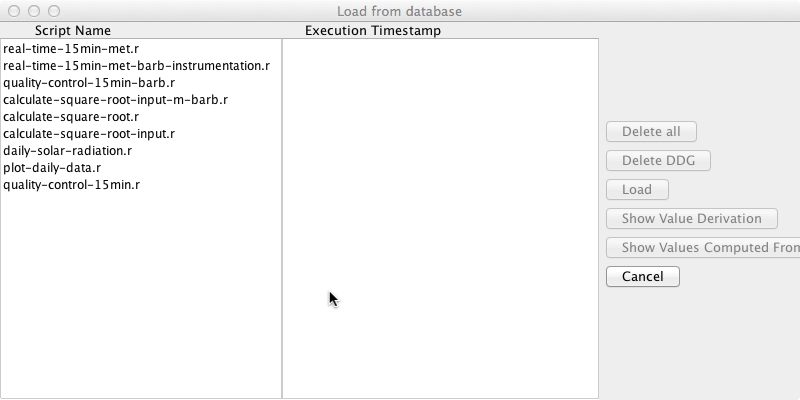
\includegraphics[width=6.5in,height=3.25in]{UsingDDGExplorer-img/UsingDDGExplorer-img005.png} 


\bigskip

{\mdseries\upshape\color{black}
The left column lists the names of scripts that have DDGs associated with them in the database. \ If you select one of these, the window will change to look like this:}

 \includegraphics[width=6.5in,height=3.25in]{UsingDDGExplorer-img/UsingDDGExplorer-img006.png} 

{\mdseries\upshape\color{black}
Now the second column shows the timestamps for all of the DDGs created from that script. \ In the rightmost column, the “Delete all” button is now enabled. \ If you click this button, it will delete all of the DDGs associated with that script from your database. \ You will be prompted to confirm that you want to delete them, but once deleted, they cannot be recovered, so be careful!}

{\mdseries\upshape\color{black}
If you select one execution timestamp, you will now see more buttons enabled:}

 \includegraphics[width=6.5in,height=3.25in]{UsingDDGExplorer-img/UsingDDGExplorer-img007.png} 

{\mdseries\upshape\color{black}
Here is what each of these buttons does.}

\liststyleWWviiiNumii
\begin{itemize}
\item {\color{black}
Delete DDG - This will delete the one DDG that corresponds to the selected script and execution timestamp after confirming that you really want to delete it.}
\item {\color{black}
Load - This will read the entire DDG from the database and create a window displaying the DDG, just as what happens when you read it from a file.}
\item {\color{black}
Show value derivation - This query allows you to view just the portion of a DDG that explains how a particular output value was calculated. \ After clicking this button, a window will appear asking you to select a variable to display. \ For example, if the user asks to see the variable 14-estimate, the (partial) DDG shown is at the right. \ Here, we can see that get.input operation outputs a number, which is input to get.random that produces the first estimate value. \ This estimate is input to calc.square.root, which produces another estimate. \ This cycle repeats until we get to the desired estimate. \ }
\begin{center}
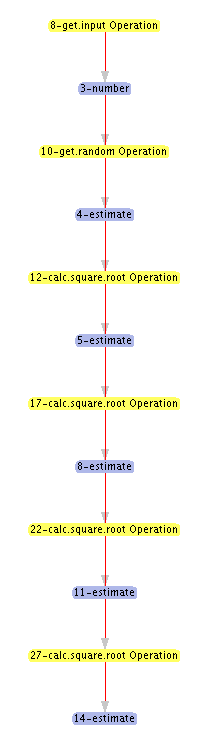
\includegraphics[width=2.2654in,height=7.8472in]{UsingDDGExplorer-img/UsingDDGExplorer-img008.png}
\end{center}
\end{itemize}
\liststyleWWviiiNumiv
\begin{itemize}
\item {\color{black}
We can get more insight by right-clicking on the data nodes to see what values they have. \ Here, we see that the 3-number has the value 3636363. \ 4-estimate has the value 3016450.69879702. \ Showing subsequent estimate values demonstrates how the algorithm narrows in on the square root value that is within the desired tolerance.}
\item \clearpage
\bigskip
\end{itemize}
\liststyleWWviiiNumv
\begin{itemize}
\item {\color{black}
Show values computed from: \ This query allows you to view the portion of the DDG that follows from a particular data value. \ After clicking this button, you will see a window like the one for the previous query where you can select a data value. \ This time, however, you will see the values that are computed from this data value as shown below.}
\end{itemize}
\liststyleWWviiiNumvi
\begin{itemize}
\item {\color{black}
Here, we start with 44-estimate and can see that it is input to two operations. \ One operation determines if it is close enough to the actual square root (which it is not), while the other uses it to refine the estimate, producing 47-estimate. \ 47-estimate is within the desired tolerance, so that value is saved in the sqr-roots.csv output file. 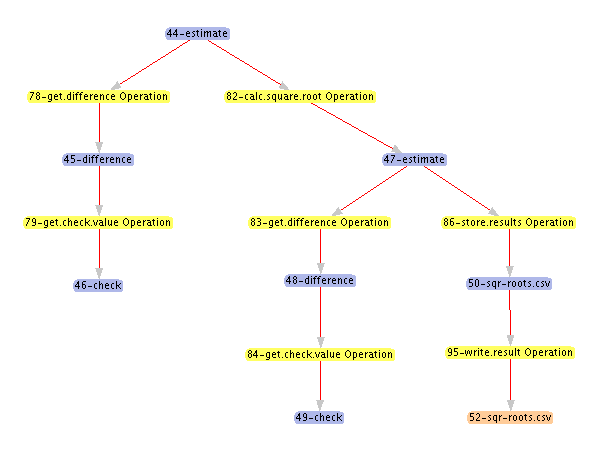
\includegraphics[width=5.8335in,height=4.4909in]{UsingDDGExplorer-img/UsingDDGExplorer-img009.png} }
\end{itemize}
\subsection{Comparing R Scripts}
{\mdseries\upshape\color{black}
You will likely find that you change your R script over time. \ The R scripts are saved in the database along with the DDG, so the DDG Explorer can always show you the R script that corresponds to a DDG.}

{\mdseries\upshape\color{black}
In addition, you may wonder how a script has changed over time, or how the script that generated one DDG differs from another script. \ To help you understand that history of your scripts, the main window of the DDG Explorer contains a button labeled “Compare R scripts”. \ When you click that, you will see this window:}

 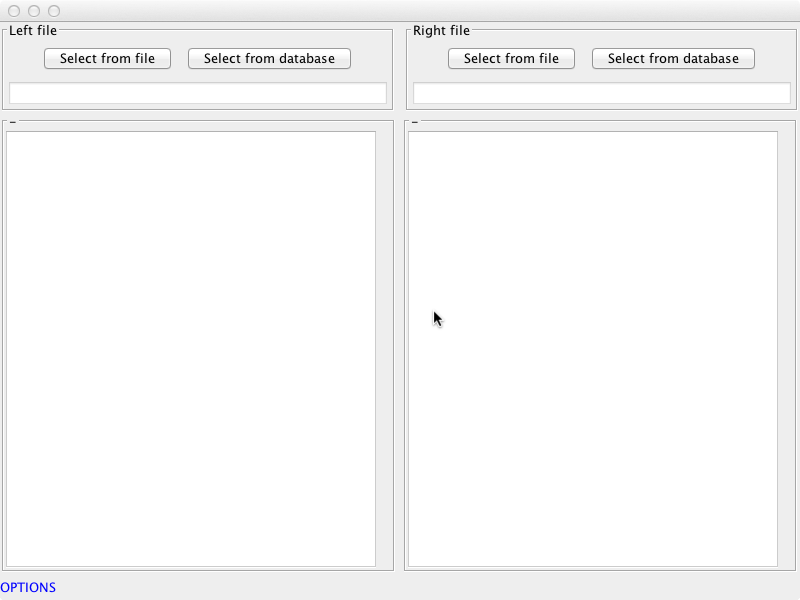
\includegraphics[width=6.5in,height=4.8752in]{UsingDDGExplorer-img/UsingDDGExplorer-img010.png} 

{\mdseries\upshape\color{black}
In this window, you can select two R scripts to compare. \ One will be displayed on the left side of the window. \ The other will be displayed on the right side of the window. \ These scripts can either come from the file system or from the database. \ }

{\mdseries\upshape\color{black}
Here is what the window will look like after selecting two related but different scripts:}

 \includegraphics[width=6.5in,height=4.8752in]{UsingDDGExplorer-img/UsingDDGExplorer-img011.png} 

{\mdseries\upshape\color{black}
The brown color identifies lines that are similar but modified between the two versions. \ Green identifies lines that have no corresponding lines in the other file. \ Red identifies places where the comparison tool has inserted blank lines just to help align the files better. \ Lines with a white background are identical between the two files.}

\subsection{Finding where Data Files are Used}
{\mdseries\upshape\color{black}
Another useful feature is to allow the user to find where a particular data file has been used as input or produced as output. \ To do that, go to the main window and click on the “Find Data Files” button. \ This will bring up the following window where you can limit the types of files searched for:}

 \includegraphics[width=6.5in,height=1.9283in]{UsingDDGExplorer-img/UsingDDGExplorer-img012.png} 

{\mdseries\upshape\color{black}
Here, you can limit to the search to just input files, just output files, or both. \ You can select one or more file extensions. \ If you select all, it will include files with any extension, including extensions not appearing in the list. \ The files are searched for in the database. \ You can either select for files appearing anywhere in the database or limit the search to a particular script or a particular ddg. \ After making your selections, another window will appear listing the matching files as follows.}

 \includegraphics[width=6.5in,height=3.25in]{UsingDDGExplorer-img/UsingDDGExplorer-img013.png} 

{\mdseries\upshape\color{black}
The first column identifies the file name. \ The second column identifies the script that used or created it. \ The third column shows the execution time of the DDG that references it. \ The last column shows the name of the node within the DDG. \ You can sort the list by clicking on the header of the column you want to sort by.}

{\mdseries\upshape\color{black}
You can now select one or more files from the list. \ After selecting files, the buttons work as follows:}

\liststyleWWviiiNumvii
\begin{itemize}
\item {\color{black}
Show Files will display the files themselves, each in a separate window.}
\item {\color{black}
Show DDGs will display the DDGS, scrolling to the position in the DDG where the file is used.}
\item {\color{black}
Compare Files will load the files using the text comparison tool. \ This will only work if exactly two files are selected. \ Currently, this button does not do anything. }
\end{itemize}
\subsection[Behind the scenes]{Behind the scenes}
{\mdseries\upshape\color{black}
This section provides some additional details on the DDG files and database.}

{\color{black}
ddg directories}

{\mdseries\upshape\color{black}
All of the information that is collected during execution of your R scripts is saved in a directory. \ It is important that you know where this directory is in order to find your DDG files and load them into the DDG Explorer.}

{\mdseries\upshape\color{black}
The directory used is the one identified by the ddg.path variable in R. \ This directory will contain a text file named ddg.txt along with files that are created by calling the instrumentation functions ddg.file, ddg.file.out, ddg.file.copy.out, ddg.snapshot, and ddg.snapshot.out. \ For details on these functions, please see the documentation on how to instrument your R code.}

{\color{black}
ddg.txt}

{\mdseries\upshape\color{black}
The ddg.txt file contains a textual definition of the DDG. \ It is not necessary to understand the contents of this file, but the interested reader can learn more by reading the Using the R DDG Library document.}

{\color{black}
DDG database}

{\mdseries\upshape\color{black}
The DDG database is stored in a directory called .ddg in your home directory. \ For example, on Windows 7, this would be something like C:{\textbackslash}Users{\textbackslash}emeryboose{\textbackslash}.ddg. \ On the Mac, this would be something like /Users/barbaralerner/.ddg. \ You should not interact with the database through the file system, but only through the DDG Explorer.}

{\color{black}
.RProfile}

{\mdseries\upshape\color{black}
The instrumentation needs to know where to find the R library. \ You can do this as follows:}

{\color{black}
ddg.library {\textless}- {\textquotedbl}c:/data/r/ddg/lib/ddg-library.r{\textquotedbl}}

{\mdseries\upshape\color{black}
source(ddg.library)}

{\mdseries\upshape\color{black}
Alternatively, you could use an environment variable to define where your library is stored. \ Doing this will make it easier to share your script with others. \ In that case, you would put this at the top of your R script.}

{\color{black}
ddg.library {\textless}- Sys.getenv(\textcolor[rgb]{0.24705882,0.24705882,0.6862745}{{\textquotedbl}DDG\_LIBRARY{\textquotedbl}})}

{\mdseries\upshape\color{black}
source(ddg.library)}

{\mdseries\upshape\color{black}
To set an environment variable, create a file called .RProfile in your home directory. \ This file should contain the following, again using the location you have chosen:}

{\color{black}
\# Tells R where to find the DDG library.}

{\mdseries\upshape\color{black}
.First {\textless}- function() \{}

{\mdseries\upshape\color{black}
\ \ \ Sys.setenv(DDG\_LIBRARY = {\textquotedbl}c:/data/r/ddg/lib/ddg-library.r{\textquotedbl})}

{\mdseries\upshape\color{black}
\}}

{\mdseries\upshape\color{black}
This function will be automatically executed whenever you start R. \ You may also find it convenient to put other commands inside the .First function that you find yourself using whenever you start R, such as a setwd call to get to your favorite working directory. }

\subsection[Acknowledgements]{Acknowledgements}
{\mdseries\upshape\color{black}
This material is based upon work supported by the National Science Foundation under Awards No. CCR-0205575, CCR-0427071, and IIS-0705772, the National Science Foundation REU grants DBI-0452254 and DBI-1003938, the Mount Holyoke Center for the Environment Summer Leadership Fellowships, and the Charles Bullard Fellowship in Forest Research at the Harvard Forest. Any opinions, findings, and conclusions or recommendations expressed in this material are those of the authors and do not necessarily reflect the views of the National Science Foundation, \ Mount Holyoke College or Harvard University.}

{\mdseries\upshape\color{black}
Numerous students have been involved in the research and tool development through the REU program at Harvard Forest, thesis research at Mount Holyoke and graduate students at the University of Massachusetts, Amherst. \ They are Cory Teshera-Sterne (Mount Holyoke and 2009 REU), Morgan Vigil (2010 REU), Sofiya Taskova (2010 REU, 2011 REU, Mount Holyoke honors thesis), Andy Galdunski (2011 REU), Garrett Rosenblatt (2011 REU), Miruna Oprescu (2012 REU), Yujia Zhou (2012 REU), Shay Addams (2013 REU), Vasco Carinhas (2013 REU), Xiang Zhao (University of Massachusetts, Amherst), Luis Antonio Perez (2014 REU), Nicole Hoffler (2014 REU) .}

{\mdseries\upshape\color{black}
Lee Osterweil from the University of Massachusetts, Amherst, Aaron Ellison and David Foster from Harvard Forest have been involved in this data provenance work for a long time and got this project started many years ago with a collaboration between UMass and Harvard Forest.}

{\mdseries\upshape\color{black}
The DDG Explorer builds on numerous packages that were developed elsewhere:}

\liststyleWWviiiNumvii
\begin{itemize}
\item {\color{black}
Little-JIL, developed at the University of Massachusetts, Amherst, under the guidance of Lee Osterweil}
\item {\color{black}
Jena, the database technology}
\item {\color{black}
Prefuse, the library used to help draw the DDGs}
\item {\color{black}
jdiff, the library that allows the comparison of R scripts. \ This is licensed by QArks.com under an LGPL license. \ The license description is available at http://www.gnu.org/licenses/lgpl.html.}
\end{itemize}
{\mdseries\upshape\color{black}
Below is the detailed licensing information that allows us to use and distribute the DDG Explorer software.}

\subsection{Jena license}
{\mdseries\upshape\color{black}
Unless otherwise noted, the following copyright statement applies:}

{\mdseries\upshape\color{black}
© Copyright 2000, 2001, 2002, 2003, 2004, 2005, 2006, 2007, 2008, 2009 Hewlett-Packard Development Company, LP}

{\mdseries\upshape\color{black}
© Copyright 2010 Talis Systems Ltd.}

{\mdseries\upshape\color{black}
© Copyright 2010 Epimorphics Ltd.}

{\mdseries\upshape\color{black}
Redistribution and use in source and binary forms, with or without modification, are permitted provided that the following conditions are met:}

{\mdseries\upshape\color{black}
Redistributions of source code must retain the above copyright notice, this list of conditions and the following disclaimer.}

{\mdseries\upshape\color{black}
Redistributions in binary form must reproduce the above copyright notice, this list of conditions and the following disclaimer in the documentation and/or other materials provided with the distribution.}

{\mdseries\upshape\color{black}
The name of the author may not be used to endorse or promote products derived from this software without specific prior written permission.}

{\mdseries\upshape\color{black}
THIS SOFTWARE IS PROVIDED BY THE AUTHOR {\textasciigrave}{\textasciigrave}AS IS'{}' AND ANY EXPRESS OR IMPLIED WARRANTIES, INCLUDING, BUT NOT LIMITED TO, THE IMPLIED WARRANTIES OF MERCHANTABILITY AND FITNESS FOR A PARTICULAR PURPOSE ARE DISCLAIMED. IN NO EVENT SHALL THE AUTHOR BE LIABLE FOR ANY DIRECT, INDIRECT, INCIDENTAL, SPECIAL, EXEMPLARY, OR CONSEQUENTIAL DAMAGES (INCLUDING, BUT NOT LIMITED TO, PROCUREMENT OF SUBSTITUTE GOODS OR SERVICES; LOSS OF USE, DATA, OR PROFITS; OR BUSINESS INTERRUPTION) HOWEVER CAUSED AND ON ANY THEORY OF LIABILITY, WHETHER IN CONTRACT, STRICT LIABILITY, OR TORT (INCLUDING NEGLIGENCE OR OTHERWISE) ARISING IN ANY WAY OUT OF THE USE OF THIS SOFTWARE, EVEN IF ADVISED OF THE POSSIBILITY OF SUCH DAMAGE.}

{\mdseries\upshape\color{black}
Jena includes software developed by the Apache Software Foundation (\url{http://www.apache.org/}).}

{\mdseries\upshape\color{black}
Jena includes RDF schemes from DCMI:}

{\mdseries\upshape\color{black}
Portions of this software may use RDF schemas Copyright (c) 2006 \href{http://dublincore.org/}{\textcolor[rgb]{0.0,0.0,0.6}{DCMI}}, the Dublin Core Metadata Initiative. These are licensed under the \href{http://creativecommons.org/licenses/by/3.0/}{\textcolor[rgb]{0.0,0.0,0.6}{Creative Commons 3.0 Attribution}} license.}

{\mdseries\upshape\color{black}
Jena is built on top of other sub-systems which we gratefully acknowledge: \href{http://jena.sourceforge.net/Licenses/index.html}{\textcolor[rgb]{0.0,0.0,0.6}{details of these systems and their version numbers}}.}

{\mdseries\upshape\color{black}
YourKit is kindly supporting open source projects with its full-featured Java Profiler. YourKit, LLC is the creator of innovative and intelligent tools for profiling Java and .NET applications. Take a look at YourKit's leading software products: \href{http://www.yourkit.com/java/profiler/index.jsp}{\textcolor[rgb]{0.0,0.0,0.6}{YourKit Java Profiler}} and \href{http://www.yourkit.com/.net/profiler/index.jsp}{\textcolor[rgb]{0.0,0.0,0.6}{YourKit .NET Profiler}}.}

\subsection{Prefuse License}
{\mdseries\upshape\color{black}
Copyright (c) 2004-2006 Regents of the University of California.}

{\mdseries\upshape\color{black}
All rights reserved.}

{\mdseries\upshape\color{black}
Redistribution and use in source and binary forms, with or without modification, are permitted provided that the following conditions are met:}

\liststyleWWviiiNumix
\begin{enumerate}
\item {\color{black}
Redistributions of source code must retain the above copyright notice, this list of conditions and the following disclaimer.}
\item {\color{black}
Redistributions in binary form must reproduce the above copyrightnotice and this list of conditions.}
\item {\color{black}
The name of the University may not be used to endorse or promote products \ \ derived from this software without specific prior written permission.}
\end{enumerate}
{\color{black}
THIS SOFTWARE IS PROVIDED BY THE REGENTS AND CONTRIBUTORS {\textasciigrave}{\textasciigrave}AS IS'{}' AND \ \ ANY EXPRESS OR IMPLIED WARRANTIES, INCLUDING, BUT NOT LIMITED TO, THE IMPLIED WARRANTIES OF MERCHANTABILITY AND FITNESS FOR A PARTICULAR PURPOSE ARE DISCLAIMED. \ IN NO EVENT SHALL THE REGENTS OR CONTRIBUTORS BE LIABLE FOR ANY DIRECT, INDIRECT, INCIDENTAL, SPECIAL, EXEMPLARY, OR CONSEQUENTIAL DAMAGES (INCLUDING, BUT NOT LIMITED TO, PROCUREMENT OF SUBSTITUTE GOODS OR SERVICES; LOSS OF USE, DATA, OR PROFITS; OR BUSINESS INTERRUPTION) HOWEVER CAUSED AND ON ANY THEORY OF LIABILITY, WHETHER IN CONTRACT, STRICT LIABILITY, OR TORT (INCLUDING NEGLIGENCE OR OTHERWISE) ARISING IN ANY WAY OUT OF THE USE OF THIS SOFTWARE, EVEN IF ADVISED OF THE POSSIBILITY OF SUCH DAMAGE.}


\bigskip
\end{document}
